\documentclass[a4paper,12pt]{article}

% Paquetes básicos
\usepackage[utf8]{inputenc}
\usepackage[T1]{fontenc}
\usepackage[spanish]{babel}
\usepackage{graphicx}
\usepackage{xcolor}
\usepackage{lipsum}
\usepackage{geometry}
\geometry{top=3cm, bottom=3cm, left=2.5cm, right=2.5cm}

% Paquetes para diseño
\usepackage{titlesec}
\usepackage{fancyhdr}
\usepackage{amsmath}
\usepackage{amssymb}
\usepackage{hyperref}

% Paquetes para el entorno lstlisting
\usepackage{listings}
\usepackage{inconsolata}

\usepackage{float}
\usepackage{enumitem}

%encabezado y pie de página nivel profesional
\usepackage{fancyhdr}
\pagestyle{fancy}
\fancyhf{}
\fancyhead[L]{\leftmark}
\fancyhead[R]{\rightmark}
\fancyfoot[C]{\thepage}
\fancyfoot[R]{\textbf{(UGR)} \today}
\renewcommand{\headrulewidth}{0.4pt}
\renewcommand{\footrulewidth}{0.4pt}
\setlength{\headheight}{15pt}
\setlength{\headsep}{10pt}
\setlength{\footskip}{20pt}
\usepackage{truncate}
\fancyhead[L]{\truncate{0.5\headwidth}{\leftmark}}
\fancyhead[R]{\truncate{0.5\headwidth}{\rightmark}}
\usepackage{mathpazo}

% Paquete para fondo
\usepackage{background}

% Configuración de lstlisting
\lstset{
    inputencoding=utf8,          % Permite UTF-8
    extendedchars=true,          % Reconoce caracteres extendidos
    literate=                    % Configuración manual para tildes y símbolos
        {á}{{\'a}}1
        {é}{{\'e}}1
        {í}{{\'i}}1
        {ó}{{\'o}}1
        {ú}{{\'u}}1
        {ñ}{{\~n}}1
        {Á}{{\'A}}1
        {É}{{\'E}}1
        {Í}{{\'I}}1
        {Ó}{{\'O}}1
        {Ú}{{\'U}}1
        {Ñ}{{\~N}}1
        {¿}{{\textquestiondown}}1
        {¡}{{\textexclamdown}}1,
    basicstyle=\ttfamily,        % Fuente monoespaciada
    breaklines=true,             % Habilita salto de línea automático
    frame=single,                % Marco alrededor del código
    backgroundcolor=\color{gray!10}, % Fondo gris claro
    keywordstyle=\color{blue},   % Color para palabras clave
    commentstyle=\color{green},  % Color para comentarios
    stringstyle=\color{red}      % Color para strings
}
\lstdefinestyle{customcpp}{
    language=C++,                % Lenguaje de programación
    showspaces=false,            % No mostrar espacios
    showtabs=false,              % No mostrar tabulaciones
    tabsize=4,                   % Tamaño de tabulación
    showstringspaces=false,      % No mostrar espacios en strings
    numbers=left,                % Números de línea a la izquierda
    numberstyle=\tiny\color{gray}, % Estilo de los números de línea
    numbersep=5pt,               % Separación de los números de línea
    stepnumber=1,                % Mostrar número en cada línea
    basicstyle=\ttfamily\footnotesize, % Estilo básico del código
    keywordstyle=\bfseries\color{blue}, % Estilo de las palabras clave
    commentstyle=\itshape\color{green!50!black}, % Estilo de los comentarios
    stringstyle=\color{red},     % Estilo de los strings
    identifierstyle=\color{black}, % Estilo de los identificadores
    % procnamekeys={def,class},    % Palabras clave para nombres de funciones
    morekeywords={constexpr,nullptr,size_t}, % Más palabras clave
    emph={int,char,double,float,unsigned}, % Palabras a enfatizar
    emphstyle=\color{magenta},   % Estilo de las palabras enfatizadas
    backgroundcolor=\color{gray!10}, % Color de fondo
    frame=shadowbox,             % Marco con sombra
    rulesepcolor=\color{gray},   % Color de la línea de separación
    breakatwhitespace=false,     % No cortar en espacios en blanco
    breaklines=true,             % Cortar líneas largas
    captionpos=b,                % Posición del título (abajo)
    escapeinside={(*@}{@*)},     % Delimitadores para escapar a LaTeX
    morecomment=[l][\color{magenta}]{\#}, % Comentarios de una línea
    morecomment=[s][\color{orange}]{/*}{*/}, % Comentarios multilínea
    morestring=[b]",             % Strings entre comillas dobles
    morestring=[b]'              % Strings entre comillas simples
}

% Configuración de título
\titleformat{\section}{\normalfont\Large\bfseries}{\thesection}{1em}{}


%definir subsubsubsection
% Paquete necesario para manipular títulos
\usepackage{titlesec}

% Definir subsubsubsection
\setcounter{secnumdepth}{4} % Aumentar el nivel de numeración
\setcounter{tocdepth}{4}    % Aumentar el nivel para la tabla de contenidos

\titleformat{\paragraph}[runin]
  {\normalfont\normalsize\bfseries}{\theparagraph}{1em}{}
\titlespacing*{\paragraph}
  {0pt}{3.25ex plus 1ex minus .2ex}{1em}

\makeatletter
\newcommand\subsubsubsection{\@startsection{paragraph}{4}{\z@}%
  {-3.25ex\@plus -1ex \@minus -.2ex}%
  {1.5ex \@plus .2ex}%
  {\normalfont\normalsize\bfseries}}
\makeatother


% Información del documento
\title{
    \vspace{-2cm}
    
\includegraphics[width=0.3\textwidth]{images/etsiit.png} \\ % Cambia el logo si es necesario
    \LARGE Ingeniería Informática + ADE\\
    \large Universidad de Granada (UGR)\\[1cm]
}
\author{\textbf{Autor:} Ismael Sallami Moreno}
\date{\textbf{Asignatura:} Apuntes Sistemas Concurrentes y Distribuidos (SCD)\\[1cm]}

% Configuración del fondo
\backgroundsetup{
    scale=1,
    color=black,
    opacity=0.2,
    angle=0,
    position=current page.south,
    vshift=0pt,
    hshift=0pt,
    contents={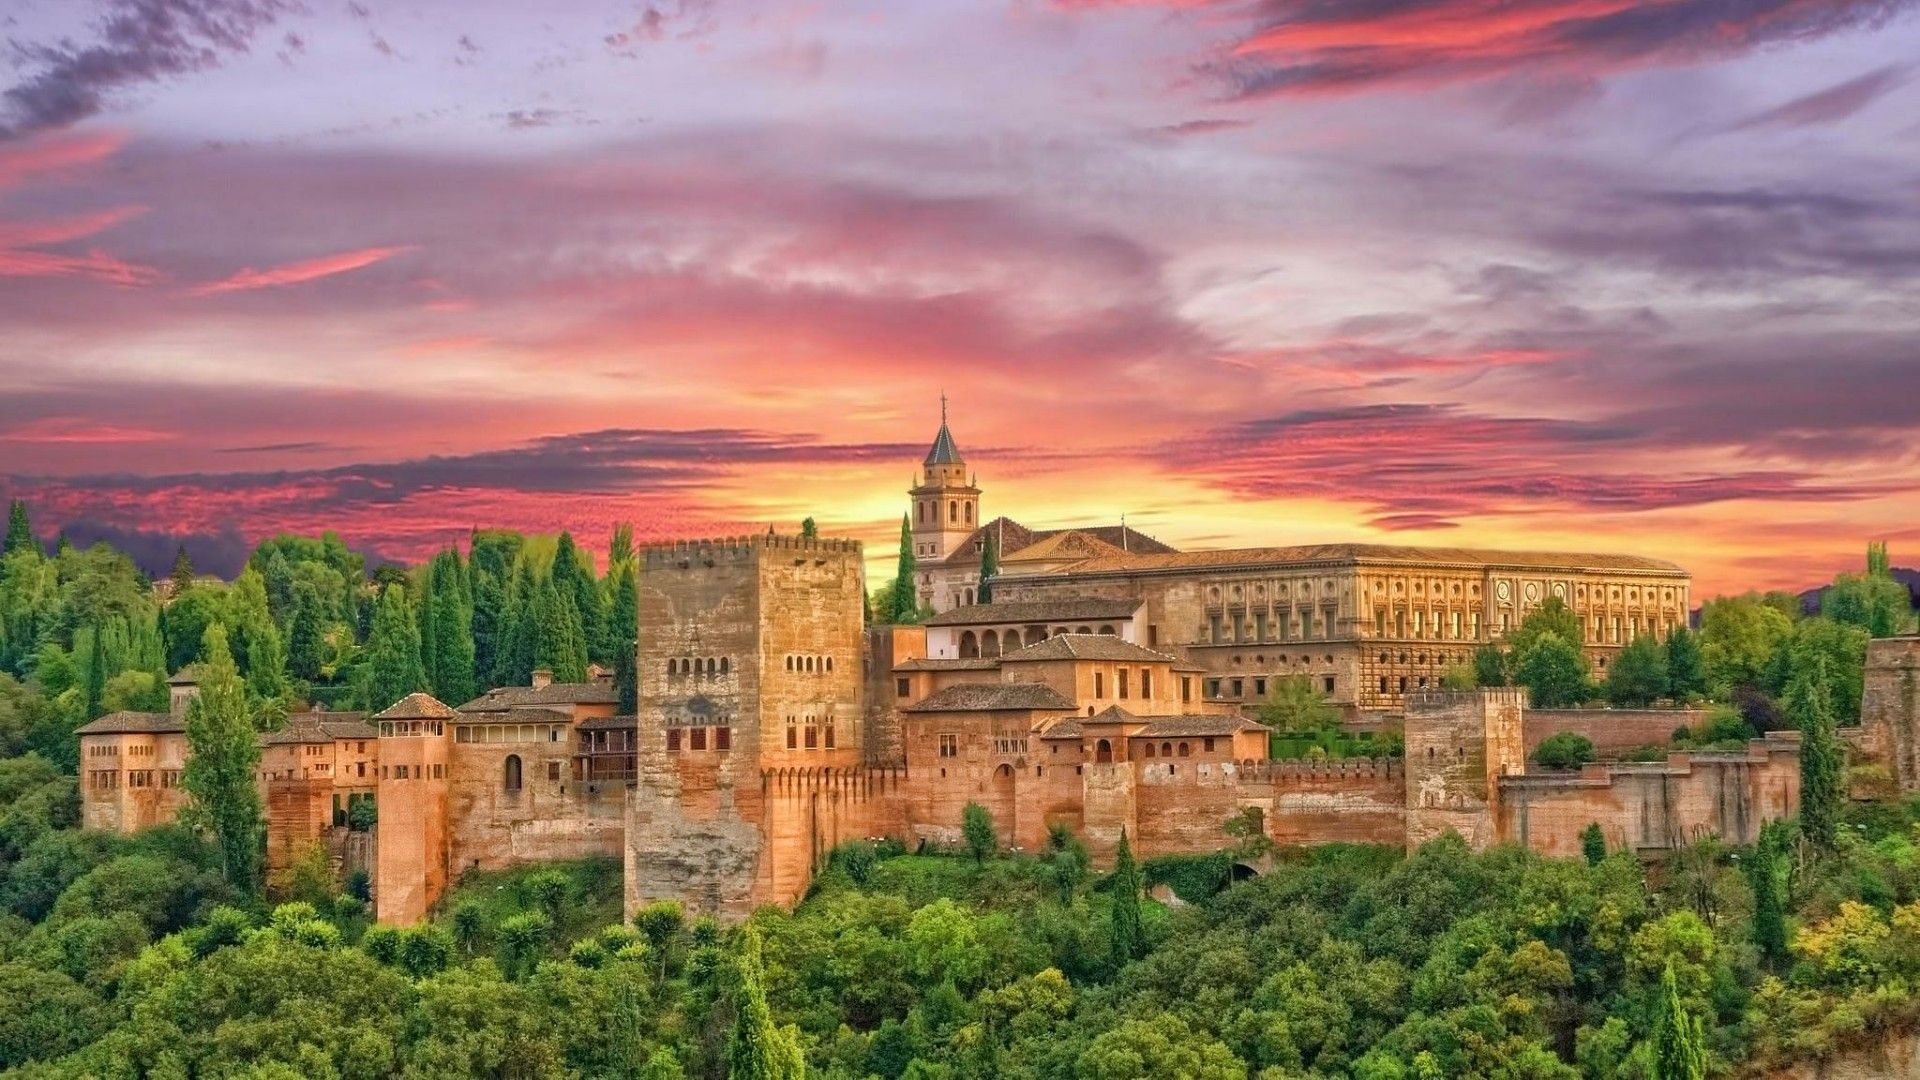
\includegraphics[width=\paperwidth,height=\paperheight,keepaspectratio]{images/granada.jpg}}
}

% Inicio del documento
\begin{document}

% Portada
\maketitle
\thispagestyle{empty}

\begin{center}
    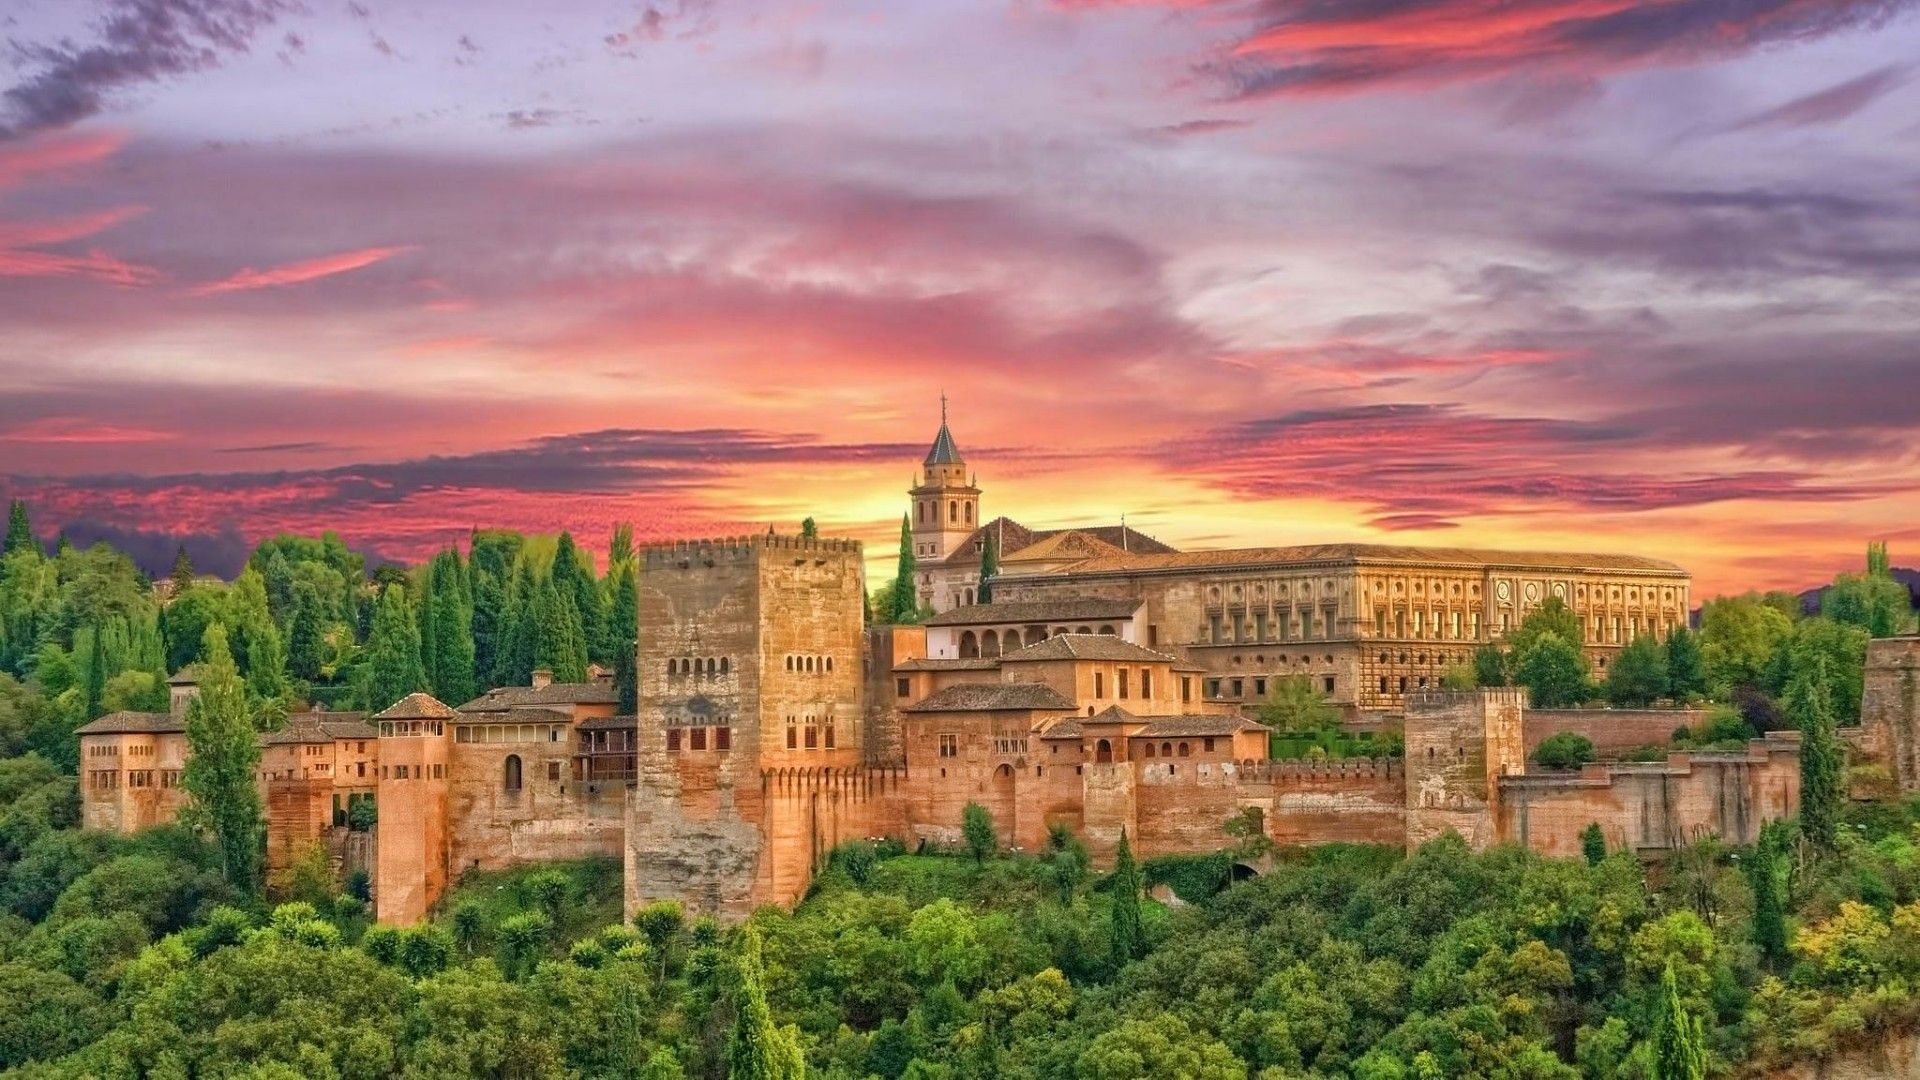
\includegraphics[width=\textwidth,height=0.4\textheight,keepaspectratio]{images/granada.jpg} \\ % Añade tu imagen de fondo
    \vfill
\end{center}

\newpage

% Índice (opcional)
\tableofcontents
\newpage

\section{Tema 3: Sistemas basados en el paso de mensajes}

\subsection{El cuello de botella de Von Neumann}

El \textbf{cuello de botella de Von Neumann} se refiere a una limitación inherente en las arquitecturas de computación clásicas basadas en el modelo de programa único almacenado. Este problema surge debido a la dependencia de un único bus para transferir datos e instrucciones entre la memoria y la unidad de procesamiento central (CPU). A continuación, se presentan sus principales características y consecuencias:

\begin{itemize}
    \item \textbf{Limitación de velocidad del bus:} La transferencia de datos entre la memoria y la CPU está restringida por la velocidad máxima del bus, lo que afecta el rendimiento general del sistema.
    \item \textbf{Cuello de botella:} Dado que no es posible realizar simultáneamente una operación de búsqueda de instrucciones y una operación de datos, se genera un retraso en el flujo de ejecución de las instrucciones.
    \item \textbf{Impacto en el rendimiento:} Esta arquitectura requiere más tiempo de ejecución para los programas, lo que reduce la eficiencia del sistema computacional.
\end{itemize}

El cuello de botella de Von Neumann es una de las razones principales por las cuales las arquitecturas modernas buscan soluciones más eficientes, como los sistemas multiprocesadores o arquitecturas paralelas.

\subsection{Clasificación de Flynn}

La \textbf{clasificación de Flynn} es un esquema que categoriza las arquitecturas de sistemas computacionales en función de cómo manejan las instrucciones y los datos durante la ejecución. Esta clasificación es fundamental para entender los diferentes modelos de procesamiento y se divide en cuatro categorías principales:

\begin{itemize}
    \item \textbf{SISD (Single Instruction, Single Data):} 
    \begin{itemize}
        \item Una sola unidad de control ejecuta una única secuencia de instrucciones.
        \item Procesa un único flujo de datos.
        \item Ejemplo: computadores monoprocesador tradicionales.
    \end{itemize}

    \item \textbf{SIMD (Single Instruction, Multiple Data):}
    \begin{itemize}
        \item Una única instrucción se aplica simultáneamente a múltiples flujos de datos.
        \item Común en aplicaciones con operaciones repetitivas sobre grandes conjuntos de datos, como gráficos y procesamiento de señales.
        \item Ejemplo: procesadores vectoriales y GPU.
    \end{itemize}

    \item \textbf{MISD (Multiple Instruction, Single Data):}
    \begin{itemize}
        \item Múltiples unidades de control ejecutan distintas instrucciones sobre un único flujo de datos.
        \item Es menos común en sistemas reales debido a limitaciones prácticas.
    \end{itemize}

    \item \textbf{MIMD (Multiple Instruction, Multiple Data):}
    \begin{itemize}
        \item Múltiples unidades de control ejecutan distintas secuencias de instrucciones sobre múltiples flujos de datos.
        \item Flexible y utilizado en sistemas paralelos modernos.
        \item Ejemplo: arquitecturas multicore y clusters de computadoras.
    \end{itemize}
\end{itemize}

Esta clasificación permite identificar las capacidades y limitaciones de las diferentes arquitecturas, sirviendo como guía para diseñar y optimizar sistemas computacionales.

%https://chatgpt.com/c/676941fc-2ae8-8012-afcb-4f356a5273ee

\subsection{Diferencias entre Multiprocesador SMP y AMP}

\begin{table}[H]
\centering
\begin{tabular}{|p{4cm}|p{6cm}|p{5cm}|}
\hline
\textbf{Características}        & \textbf{SMP (Multiprocesamiento Simétrico)}  & \textbf{AMP (Multiprocesamiento Asimétrico)}  \\ \hline
\textbf{Arquitectura}           & Todos los procesadores son iguales y comparten el acceso a la memoria & Un procesador principal controla el sistema y los otros son secundarios  \\ \hline
\textbf{Acceso a memoria}       & Todos los procesadores tienen acceso compartido a la memoria central  & Solo el procesador principal tiene acceso a la memoria central  \\ \hline
\textbf{Control de procesos}    & Los procesadores pueden trabajar independientemente & El procesador principal gestiona los procesos y asigna tareas a los secundarios \\ \hline
\textbf{Escalabilidad}          & Alta escalabilidad; se pueden agregar más procesadores sin mucha complicación  & Baja escalabilidad; añadir más procesadores no mejora el rendimiento de forma eficiente \\ \hline
\textbf{Costo}                  & Más costoso debido a la necesidad de múltiples procesadores iguales y una memoria compartida  & Menos costoso, ya que solo se necesita un procesador principal y algunos secundarios \\ \hline
\textbf{Rendimiento}            & Mejor rendimiento en tareas paralelas y de procesamiento intensivo  & Menor rendimiento en tareas paralelas, debido a la dependencia del procesador principal \\ \hline
\textbf{Sistemas típicos}       & Servidores, estaciones de trabajo y sistemas de alta gama  & Sistemas embebidos, estaciones de trabajo de menor escala y dispositivos con recursos limitados \\ \hline
\end{tabular}
\caption{Diferencias entre Multiprocesador SMP y AMP}
\end{table}


\subsection{Mecanismo de citas}

Se trata de una operación de comunicación NO bloqueante y sin búfer. La cita tiene lugar antes de que comience la transmisión de datos.

\subsection{Paso de mensajes bloqueante con búfer}

El proceso emisor vuelve inmediatamente al ejecutar la operación de envío, \textit{salvo que el proceso buffer esté lleno}. En este caso, el proceso emisor se bloquea hasta que haya espacio en el buffer. La operación \textit{receive} no vuelve hasta que se han recibido los datos.

\subsection{Paso de mensajes no bloqueante con búfer}

En este caso se reduce el tiempo de espera debido a que la operación \textit{receive} provoca la transferencia inmediata de datos del búfer a la memoria del proceso receptor.

\subsection{MPI}
\subsubsection{Comunicación bloqueante}
\subsubsection*{Campos de operación MPI de envío con buffer}
\begin{lstlisting}[language=c++]
int MPI_Send(void *buf, int count, MPI_Datatype datatype, int dest, int tag, MPI_Comm comm);
\end{lstlisting}
\subsubsection*{Campos de operación MPI de recepción con buffer}
\begin{lstlisting}[language=c++]
int MPI_Recv(void *buf, int count, MPI_Datatype datatype, int source, int tag, MPI_Comm comm, MPI_Status *status);
\end{lstlisting}

\begin{itemize}
    \item El \textit{origen, tag, comunicador} deben de coincidir en el mensaje enviado y recibido.
    \item \textit{MPI\_Send, MPI\_Recv, MPI\_Ssend} no vuelven hasta que se completan.
\end{itemize}

\subsubsection{Comunicación No bloqueante}
\begin{itemize}
    \item \textit{MPI\_Isend, MPI\_Irecv, MPI\_Iprobe, MPI\_Test} son operaciones no bloqueantes.
\begin{itemize}
    \item \textit{MPI\_Isend:} Inicia una operación de envío no bloqueante. Permite que el programa continúe ejecutándose mientras se realiza la operación de envío en segundo plano.
    \item \textit{MPI\_Irecv:} Inicia una operación de recepción no bloqueante. Permite que el programa continúe ejecutándose mientras se realiza la operación de recepción en segundo plano.
    \item \textit{MPI\_Iprobe:} Permite comprobar de manera no bloqueante si hay un mensaje disponible para ser recibido. Esto es útil para evitar que el programa se bloquee esperando un mensaje.
    \item \textit{MPI\_Test:} Verifica si una operación no bloqueante ha completado. Esto permite al programa comprobar el estado de las operaciones no bloqueantes y actuar en consecuencia.
\end{itemize}
\end{itemize}

\subsubsection{Sondeo de Mensajes}
\begin{itemize}
    \item \textit{MPI\_Iprobe} y \textit{MPI\_Probe} son operaciones de sondeo de mensajes que permiten a un proceso verificar si hay mensajes disponibles para ser recibidos.
    \begin{itemize}
        \item \textit{MPI\_Iprobe:} Permite sondear de manera no bloqueante si hay mensajes disponibles para ser recibidos. Devuelve un valor verdadero si hay mensajes pendientes y falso en caso contrario. El valor que modifica es el flag, es decir, si flag>0, hay que recibirlo con MPI\_Recv, debido a que se da la existencia de un mensaje no bloqueante.
        \item \textit{MPI\_Probe:} Permite sondear de manera bloqueante si hay mensajes disponibles para ser recibidos. Se bloquea hasta que llega un mensaje.
    \end{itemize}
\end{itemize}

\subsection*{Diferencias entre MPI\_Probe y MPI\_IProbe}

\begin{table}[ht]
\centering
\begin{tabular}{|p{5cm}|p{5cm}|p{5cm}|}
\hline
\textbf{Característica}        & \textbf{MPI\_Probe} & \textbf{MPI\_IProbe}  \\ \hline
\textbf{Bloqueante}           & Sí & No  \\ \hline
\textbf{Comportamiento}       & Espera hasta que haya un mensaje disponible & Vuelve inmediatamente con el estado del mensaje  \\ \hline
\textbf{Eficiencia}           & Puede causar ineficiencia en ausencia de mensajes mientras se espera & Permite trabajar en paralelo mientras se espera  \\ \hline
\end{tabular}
\caption{Diferencias entre MPI\_Probe y MPI\_IProbe}
\end{table}

\subsection{Explicación del código de la criba de Eratóstenes}

Para ello pincha \href{https://github.com/ElblogdeIsmael/ElblogdeIsmael.github.io/blob/main/Asignaturas/Tercer%20A%C3%B1o/SCD/Resumenes/ETSIIT/cribaExplicacion.md}{aquí}. Además la actividad extra se encuentra \href{https://github.com/ElblogdeIsmael/ElblogdeIsmael.github.io/blob/main/Asignaturas/Tercer%20A%C3%B1o/SCD/Teoria/Actividad_Extra/cribadeErastotenes/ETSIIT/build/Erastotenes.pdf}{aquí}.


\subsubsection{Explicación del problema del museo}

\begin{lstlisting}[style = customcpp]
    PUERTA(i:1..2)::
{ int s=0;
do
if (s<HORA.CIERRE && PERSONA())->
{send(CONTROL, S()); //envia una se\~nal de entrada
de persona
DELAY.UNTIL(s+1);//espera hasta el siguiente
instante
s:=s+1;// cuenta un nuevo tick de reloj
}
[]
(s<HORA.CIERRE && NOT PERSONA())->
DELAY.UNTIL(s+1);//espera hasta el siguiente
instante
s:=s+1;]//cuenta otro tick
[]
TRUE->DELAY.UNTIL (TIME() + 16*3600);
//es la hora de cierre del museo; hay
//que esperar 16 horas para activar el controlador
.
// TIME() devuelve una cuenta en segundos.
fi
do;
send(CONTROL, Start();}
CONTROL::
{ int cont= 0;
if receive(PUERTA(1), Start());
//desde cualquiera de los sensores
[] //de las puertas se arranca
receive(PUERTA(2), Start());//el controlador
fi
do
[]*[(j:1..2) receive(PUERTA(j), S())-> cont:= cont
+1];
//cuenta una persona mas, porque ha recibido la se\~nal
//de cualquiera de las 2 puertas (no se puede saber cual)
od;
printf("numero de personas", %d, cont));
}
main(){
cobegin PUERTA;CONTROL coend;}
\end{lstlisting}

\subsection{Orden Select}
\begin{itemize}
    \item versión de orden alternativa no determinista
    \item modo síncrono de comunicación, paso de mensajes bloqueantes
    \item resuelve el problema de la recepción de tener varias variables pendientes sin dependencias del orden temporal
\end{itemize}

\subsubsection{Semántica de la orden select}
\begin{itemize}
    \item cada bloque que comienza con \textit{when} se denomina alternativa (orden guarda)
    \item desde when hasta do se denomina guarda de dicha alternativa
    \item instrucciones receive nombran a otros procesos del programa concurrente y cada uno referencia a una variable local
\end{itemize}
\begin{lstlisting}[style=customcpp]
    select
when condicion1 receive( variable1, proceso1 ) do
sentencias1
when condicion2 receive( variable2, proceso2 ) do
sentencias2
...
when condicionn receive( variablen, proceson ) do
sentenciasn
end
\end{lstlisting}

\subsubsection{Formas de poner la guarda de una orden select}

\begin{itemize}
    \item when receive(mensaje, proceso) do sentencias 
    \item when true receive(mensaje, proceso) do sentencias
    \item when condicion do sentencias (puede omitirse el receive, decimos que es una guarda sin sentencia de entrada)
\end{itemize}

\subsubsection{Tipos de ejecución de las guardas}
\begin{itemize}
    \item guarda ejecutable: si la condición es verdadera y ya ha iniciado la sentencia send
    \item guarda potencialmente ejecutable: si la condición es verdadera pero no ha iniciado la sentencia send
    \item guarda no ejecutable
\end{itemize}

\subsubsection{Determinación de la guarda a ejecutar}
\begin{itemize}
    \item aquella que inicio el send antes
    \item se selecciona no determinísticamente una cualquiera si no hay guardas con sentencias de entrada
    \item si hay solo guardas potenciablemente ejecutables, se inicia la guarda cuando esta inicia la sentencia send
    \item si no hay ningún tipo de guarda se genera una excepción/error.
\end{itemize}

Hay que tener en cuenta que la ejecución de un instrucción select conlleva esperas, por lo que pueden producirse situaciones de interbloqueo.\\

Existe una orden select con prioridad, por lo que dejaría de ser no determinística.\\

Para programar a un servicio servidor se debe de ejecutar el select dentro de un bucle para que se evalúe de nuevo la guarda y se seleccione no determinísticamente a una de ellas para poder ejecutarlas.

\subsubsection{Ejemplo: Productor-Consumidor con Búfer FIFO}

Este ejemplo ilustra el patrón clásico de \textbf{productor-consumidor} utilizando un búfer FIFO intermedio. En este esquema:

\begin{itemize}
    \item El \textbf{productor} genera elementos y los envía al búfer.
    \item El \textbf{intermedio} actúa como un búfer que controla la inserción y extracción de datos, garantizando condiciones de sincronización mediante guardas.
    \item El \textbf{consumidor} extrae elementos del búfer y los procesa.
\end{itemize}

La clave de este diseño radica en que el intermedio no conoce de antemano el orden de las peticiones de inserción y extracción, pero asegura la propiedad de \textbf{seguridad} en el acceso concurrente al búfer.

\begin{lstlisting}[style=customcpp, caption={Productor-Consumidor con Búfer FIFO}, label={lst:prod-cons}]
    { Productor (P) }
    while true do                        // Inicia un bucle infinito en el productor.
    begin
        v := Produce();                  // El productor genera un valor 'v'.
        s_send(v, B);                    // El productor envía el valor 'v' al búfer 'B'.
    end
    
    { Intermedio (B) }
    var esc, lec, cont: integer := 0;    // Inicializa las variables: 'esc' (índice de escritura), 'lec' (índice de lectura) y 'cont' (contador de elementos en el búfer).
    buf: array[0..tam-1] of integer;    // Declara el búfer 'buf' como un arreglo de tamaño 'tam', donde se almacenarán los valores producidos.
    begin
        while true do                    // Inicia un bucle infinito en el intermedio (el búfer).
            select                         // Comienza una selección de condiciones para ser ejecutadas.
                when cont < tam receive(v, P) do       // Si el número de elementos en el búfer es menor que 'tam', hay espacio para almacenar más elementos, El intermedio recibe un valor 'v' del productor (P).

                    buf[esc] := v;        // El valor recibido se almacena en la posición 'esc' del búfer.
                    esc := (esc + 1) mod tam;  // Se actualiza el índice de escritura 'esc' de manera circular (se vuelve a 0 cuando alcanza 'tam').
                    cont := cont + 1;     // Se incrementa el contador de elementos en el búfer.
                when 0 < cont receive(s, C) do             // Si el número de elementos en el búfer es mayor que 0, hay datos para consumir, El intermedio recibe una solicitud del consumidor (C).

                    s_send(buf[lec], C);  // El intermedio envía el valor almacenado en 'lec' al consumidor.
                    lec := (lec + 1) mod tam;  // Se actualiza el índice de lectura 'lec' de manera circular.
                    cont := cont - 1;     // Se decrementa el contador de elementos en el búfer.
            end
    end
    
    { Consumidor (C) }
    while true do                        // Inicia un bucle infinito en el consumidor.
    begin
        s_send(s, B);                    // El consumidor solicita un valor del búfer (envía una solicitud 's' al búfer).
        receive(v, B);                   // El consumidor recibe el valor 'v' del búfer.
        Consume(v);                      // El consumidor procesa el valor recibido.
    end
\end{lstlisting}


    
    

%explicacion
\subsubsection*{Breve Explicación}

\begin{itemize}
    \item \textbf{Productor (P):} Un bucle infinito genera valores (\textit{Produce}) y los envía al búfer (\textit{s\_send(v, B)}).
    \item \textbf{Intermedio (B):} Administra las operaciones de inserción y extracción usando un arreglo cíclico:
    \begin{itemize}
        \item Inserta valores en el búfer si no está lleno (\textit{cont < tam}).
        \item Extrae valores del búfer si no está vacío (\textit{cont > 0}).
        \item Las guardas en las sentencias \textit{select} controlan estas condiciones.
    \end{itemize}
    \item \textbf{Consumidor (C):} Recibe valores del búfer y los consume (\textit{Consume(v)}).
\end{itemize}

Este modelo asegura la sincronización entre los procesos mediante las condiciones de las guardas, evitando inconsistencias en el acceso concurrente al búfer.


\subsubsection{Select con Guardas Indexadas}

\textbf{Instrucción \texttt{Select} con guardas indexadas}  
Cuando es necesario replicar alternativas en una estructura de espera selectiva, se puede utilizar una construcción que evita la redundancia de código. La sintaxis para lograrlo es:

\begin{lstlisting}[style=customcpp]
for indice := inicial to final
when condicion receive(mensaje, proceso) do
    sentencias(indice);
\end{lstlisting}

En esta construcción, tanto la condición, el mensaje, el proceso y las sentencias pueden referirse al índice de la iteración. Esta forma compacta es equivalente a expandir explícitamente las alternativas, como se muestra a continuación:

\begin{lstlisting}[style=customcpp]
when condicion receive(mensaje, proceso) do
    sentencias { se sustituye indice por inicial }
when condicion receive(mensaje, proceso) do
    sentencias { se sustituye indice por inicial + 1 }
...
\end{lstlisting}

Este mecanismo facilita la creación de programas distribuidos más legibles y eficientes, reduciendo la redundancia en el código fuente.


\subsubsection{Select con sentencia else}

En este caso es similar al uso del \textit{when}, pero en este caso debemos de hacer uso del \textit{else}, podemos concebir que el uso y desempeño es similar al de in if\-else, pero en este caso es un when\-else. Ejemplo:
\begin{lstlisting}[style=customcpp, caption={Select con sentencia else}, label={lst:select-else}]
    // Declaración de variables globales
    var suma : array[0..n-1] of integer := (0,0,...,0) ; // Arreglo para almacenar las sumas parciales de cada proceso.
    continuar : boolean := true ;                       // Variable de control para el bucle principal.
    numero : integer ;                                  // Variable para recibir el número enviado por un proceso.
    
    begin
    while continuar do begin                            // Bucle principal que se ejecuta mientras 'continuar' sea verdadero.
        select                                           // Inicia la estructura de selección para manejar múltiples condiciones.
            for i := 0 to n - 1                         // Itera sobre todos los procesos del 0 al n-1.
            when suma[i] < 100 receive( numero, emisor[i] ) // Si la suma parcial del proceso i es menor que 100,
                                                             // recibe un número de dicho proceso (emisor[i]).
            do
                suma[i] := suma[i] + numero ;            // Actualiza la suma parcial del proceso i con el número recibido.
                continuar := true ;                      // Establece 'continuar' como verdadero para seguir ejecutando el bucle.
                                                          // Nota: esta instrucción no es estrictamente necesaria, pero aclara
                                                          // que el bucle continuará.
        end
        else continuar := false;                        // Si no se cumple ninguna condición, establece 'continuar' como falso
                                                        // para salir del bucle principal.
    end
    end
\end{lstlisting}
    








%https://chatgpt.com/c/676941fc-2ae8-8012-afcb-4f356a5273ee---4o
%https://chatgpt.com/c/676ae4b6-51a8-8012-a6fb-f0bf91751044---normal

\section{Tema 4: Introducción a los Sistemas de Tiempo Real}

\subsection{Confusión con otros sistemas}

Los sistemas de tiempo real (STR) a menudo se confunden con otros tipos de sistemas debido a ciertas similitudes en sus características y comportamientos. A continuación, se explican las razones de estas confusiones:

\begin{itemize}
    \item \textbf{En línea:} Los sistemas en línea están diseñados para estar disponibles y operativos en todo momento, similar a los STR que deben responder a eventos en tiempo real. Sin embargo, la diferencia clave es que los STR tienen restricciones temporales estrictas que deben cumplirse para garantizar el correcto funcionamiento del sistema.
    \item \textbf{Interactivos:} Los sistemas interactivos permiten la interacción directa con los usuarios, lo que puede dar la impresión de que son sistemas de tiempo real. No obstante, los STR no solo requieren interacción, sino que también deben cumplir con plazos específicos para procesar y responder a eventos.
    \item \textbf{Rápidos:} La velocidad de respuesta es una característica común tanto en sistemas rápidos como en STR. Sin embargo, la principal diferencia radica en que los STR no solo deben ser rápidos, sino que deben garantizar que las respuestas ocurran dentro de un tiempo predefinido y crítico para el correcto funcionamiento del sistema.
\end{itemize}

\subsection{Propiedades de los STR}

Los Sistemas de Tiempo Real (STR) tienen ciertas propiedades fundamentales que los distinguen de otros sistemas informáticos. Estas propiedades son esenciales para asegurar que los STR cumplan con los requisitos temporales y de fiabilidad en su funcionamiento. Las principales propiedades de los STR son las siguientes:

\begin{itemize}
    \item \textbf{Reactividad:} Los sistemas de tiempo real deben reaccionar de manera adecuada y rápida a los eventos que ocurren en el entorno. La reactividad implica que el sistema debe responder a los eventos en un tiempo predecible, es decir, la respuesta no solo depende de lo que el sistema haga, sino también de cuándo lo haga. Esta propiedad es crucial en aplicaciones como el control de sistemas de vuelo o los sistemas de frenado en vehículos.
    
    \item \textbf{Determinismo:} Un STR debe ser determinista, lo que significa que dada una entrada específica, el sistema debe producir siempre la misma salida dentro de un tiempo determinado. El comportamiento de un STR es predecible y se puede calcular con antelación. Esto es fundamental en sistemas como los de control de maquinaria, donde la predictibilidad es crucial para garantizar el buen funcionamiento del sistema sin errores inesperados.
    
    \item \textbf{Responsabilidad:} Esta propiedad hace referencia a la capacidad de un STR para garantizar que las tareas o procesos se completan dentro de sus plazos establecidos. En otras palabras, un STR debe ser capaz de asegurar que las tareas se ejecuten correctamente y a tiempo, incluso bajo condiciones de carga alta o en situaciones imprevistas. La responsabilidad es vital para garantizar la estabilidad y efectividad del sistema.
    
    \item \textbf{Confiabilidad:} Los STR deben ser confiables, lo que significa que deben funcionar correctamente y de forma estable durante su operación, incluso ante fallos o errores. La confiabilidad es una propiedad clave para sistemas críticos como los utilizados en aplicaciones médicas, aeronáuticas o automotrices, donde un fallo podría tener consecuencias graves. La fiabilidad implica que los sistemas estén diseñados para manejar fallos de manera segura o minimizar su impacto.
\end{itemize}

\subsection{Definición en el ámbito de los sistemas operativos}

Sistema Operativo de Tiempo Real es aquel que tiene la capacidad para suministrar un nivel de servicio requerido en un tiempo limitado y especificado a priori.

\subsection{Clasificación de los STR}

Los Sistemas de Tiempo Real (STR) se pueden clasificar según el nivel de criticidad temporal que tienen sus tareas, lo cual influye en los requisitos y características de cada sistema. A continuación, se presentan tres categorías basadas en la criticidad de los STR:

\subsubsection{Atendiendo a la criticidad de los STR}

\begin{itemize}
    \item \textbf{Misión Crítica:} Estos sistemas son los más críticos, ya que cualquier fallo en la ejecución dentro del tiempo establecido puede tener consecuencias graves. Un ejemplo de este tipo de sistema es el \textit{control de aterrizaje} de aeronaves, donde la puntualidad y exactitud son cruciales para la seguridad de la operación. Los complementos importantes en estos sistemas incluyen \textit{tolerancia a fallos}, lo que significa que el sistema debe ser capaz de manejar y recuperarse de errores sin comprometer la seguridad ni la efectividad.
    
    \item \textbf{Estrictos:} Los sistemas estrictos también requieren una alta precisión temporal, aunque las consecuencias de un fallo no son tan críticas como en los sistemas de misión crítica. Un ejemplo sería el sistema de \textit{reservas de vuelos}, donde las respuestas deben ser rápidas y dentro de los tiempos previstos, pero un pequeño retraso no implica necesariamente un fallo catastrófico. Los complementos asociados a estos sistemas incluyen \textit{calidad de la respuesta}, ya que es importante que la respuesta no solo sea puntual, sino que también sea precisa y eficiente.
    
    \item \textbf{Permisivos:} Estos sistemas tienen requisitos menos estrictos en cuanto a tiempo, ya que las tareas pueden tolerar ciertos retrasos sin consecuencias graves. Un ejemplo típico sería la \textit{adquisición de datos meteorológicos}, donde los datos pueden ser procesados con algo de retraso sin que afecte gravemente al resultado final. Los complementos de estos sistemas incluyen \textit{medidas de fiabilidad}, lo que significa que, aunque el sistema no necesite ser extremadamente puntual, debe ser confiable y eficiente en su funcionamiento.
\end{itemize}

\subsection{Tipos de medidas del tiempo de interés en STR}

Existen dos tipos principales de medidas del tiempo de interés en los Sistemas de Tiempo Real (STR): el \textbf{tiempo absoluto} y los \textbf{intervalos o tiempo relativo}. A continuación se detallan ambos tipos:

\subsubsection{1. Tiempo Absoluto}
El tiempo absoluto se refiere a la medición del tiempo con relación a un sistema de referencia global. Algunos de los sistemas de referencia más comunes incluyen:

\begin{itemize}
    \item \textbf{Sistemas de referencia locales:} Este tipo de medida usa un sistema de tiempo basado en la localización geográfica de un lugar específico. Puede estar basado en relojes locales o sistemas de referencia regionales.
    
    \item \textbf{Astronómicos (UT0):} Se refiere al tiempo universal basado en la rotación de la Tierra en relación con las estrellas. El \textit{UT0} es un tiempo que considera los movimientos irregulares de la Tierra y es usado como una medida precisa en astronomía.
    
    \item \textbf{Atómicos (IAT):} El Tiempo Atómico Internacional (IAT) es una medida basada en la oscilación de los átomos de cesio y es utilizado para obtener un estándar muy preciso de medición del tiempo. Este tiempo es utilizado como base para el UTC.
    
    \item \textbf{Tiempo Coordinado Universal (UTC):} Es el estándar internacional de tiempo utilizado para coordinar el tiempo globalmente. Desde 1972, el UTC ha sido utilizado ampliamente y es una medida combinada basada en el IAT, pero con ajustes ocasionales para sincronizarlo con la rotación de la Tierra.
    
    \item \textbf{Satelital (GPS):} El tiempo de GPS (GPST) es una escala de tiempo continua que no tiene segundos intercalares. Se define a partir del segmento de control del sistema GPS, el cual se basa en relojes atómicos ubicados en estaciones de monitoreo y en los satélites. Este sistema comenzó a las 00:00 UTC del 5 al 6 de enero de 1980.
\end{itemize}

\subsubsection{2. Intervalos o Tiempo Relativo}
El tiempo relativo se refiere a la medición de intervalos de tiempo entre eventos, y no a un instante específico en un sistema de referencia global. Los intervalos de tiempo pueden no ser monótonos, lo que significa que pueden verse afectados por factores como la deriva o los ajustes de reloj. En STR, esto es importante porque el tiempo computacional puede no ser uniforme o estable debido a la interferencia de diferentes tareas en ejecución.

Por ejemplo, el \textit{Tiempo Computador} puede variar dependiendo de la carga del sistema, lo que hace que el tiempo sea no monótono, y este comportamiento debe ser gestionado adecuadamente para garantizar el cumplimiento de los plazos de las tareas en los STR.





La medida del tiempo en los Sistemas de Tiempo Real (STR) se realiza a través de diferentes tipos de relojes y características que permiten un seguimiento preciso de los eventos y tareas dentro de los sistemas. A continuación se presentan los conceptos clave y características de los relojes de tiempo real:

\subsubsection{Concepto de reloj de tiempo real}
El reloj de tiempo real puede estar basado en diferentes componentes que permiten su funcionamiento:

\begin{itemize}
    \item \textbf{Oscilador:} Es un dispositivo que genera una señal de frecuencia constante, utilizada para medir el tiempo. Los osciladores suelen ser muy precisos, pero pueden tener limitaciones en cuanto a estabilidad a largo plazo.
    \item \textbf{Contador:} Un contador de tiempo real lleva el registro del tiempo mediante una secuencia de pulsos. Cada pulso representa una unidad de tiempo y el contador se incrementa con cada uno. Este tipo de reloj puede ser más eficiente en cuanto a precisión temporal.
    \item \textbf{Software:} Los relojes de tiempo real basados en software utilizan el sistema operativo y el hardware subyacente para realizar mediciones temporales. Estos pueden estar sujetos a variaciones o retardos dependiendo de las cargas de trabajo del sistema.
\end{itemize}

\subsubsection{Características más importantes de los relojes de tiempo real}

Los relojes de tiempo real tienen características fundamentales que permiten su funcionamiento adecuado en los STR:

\begin{itemize}
    \item \textbf{Precisión (granularidad):} La precisión de un reloj de tiempo real se refiere a la mínima unidad de tiempo que puede medir. Esta se mide generalmente en nanosegundos (ns), microsegundos (\(\mu\)s), milisegundos (ms), o segundos (s). Cuanto mayor sea la precisión, mayor será la capacidad del sistema para gestionar tareas con plazos muy estrictos.
    
    \item \textbf{Tiempo de desbordamiento:} El tiempo de desbordamiento se refiere al límite de tiempo después del cual un contador o reloj vuelve a cero. Este comportamiento es común en relojes de 32 bits, ya que al llegar al límite de valor, el contador se reinicia.
    
    \item \textbf{Intervalo:} El intervalo se refiere al tiempo transcurrido entre dos eventos consecutivos o dos mediciones del reloj. Este intervalo puede ser afectado por la precisión del reloj y la estabilidad del sistema.
\end{itemize}

\subsubsection{Escalas temporales}
Existen varias escalas temporales utilizadas en los STR, dependiendo del tipo de medición y de las necesidades de la aplicación. Algunas de las más comunes son:

\begin{itemize}
    \item \textbf{Tiempo monótono:} Es un tipo de tiempo en el que el reloj avanza de manera continua, sin retroceder o saltar en el tiempo. Es muy útil para aplicaciones que requieren un seguimiento constante del tiempo.
    
    \item \textbf{Tiempo no monótono:} En este caso, el reloj puede avanzar o retroceder en función de varios factores, como ajustes de los relojes o cambios de sistema. Es común en sistemas que necesitan sincronización con otros sistemas o eventos externos, como los relojes GPS.
    
    \item \textbf{Tiempo absoluto:} Es un tiempo basado en un sistema de referencia global (por ejemplo, UTC), que no depende de los eventos o el sistema local.
    
    \item \textbf{Tiempo no absoluto:} El tiempo no absoluto depende del sistema local y puede estar sujeto a variaciones o desincronización respecto a un sistema de referencia global.
\end{itemize}

\subsubsection{Precisión y Intervalo para un contador de 32 bits}

A continuación se muestra la relación entre la precisión y el intervalo para un contador de 32 bits. Este tipo de contador tiene una capacidad limitada debido al tamaño del número que puede almacenar (32 bits), lo que implica que el contador se desbordará después de un determinado intervalo.

\begin{itemize}
    \item \textbf{Precisión:} La precisión de un contador de 32 bits puede variar dependiendo de la unidad de medida. A continuación se presentan algunos ejemplos de intervalos de tiempo que un contador de 32 bits puede manejar:
    \begin{itemize}
        \item 100 ns (nanosegundos) hasta 429,5 segundos.
        \item 1 \(\mu\)s (microsegundos) hasta 71,58 minutos.
        \item 100 \(\mu\)s (microsegundos) hasta 119,3 horas.
        \item 1 ms (milisegundos) hasta 49,71 días.
        \item 1 s (segundo) hasta 136,18 años.
    \end{itemize}
    
    Estos valores indican el intervalo máximo que un contador de 32 bits puede medir antes de que se produzca un desbordamiento. Cuanto mayor sea la precisión, menor será el intervalo que el contador podrá gestionar antes de desbordarse.
\end{itemize}





\subsection{Temporizadores}

Los temporizadores son elementos clave en los sistemas operativos y en los sistemas concurrentes y distribuidos, particularmente en sistemas de tiempo real. A continuación, se describen sus características y cómo se utilizan para gestionar el tiempo y las tareas dentro del sistema.

\subsubsection{Ideas Fundamentales}

Los temporizadores no son instrucciones nativas de los lenguajes de programación, sino que se activan mediante una llamada o operación de sistema operativo. Funcionan como relojes especializados en la gestión de tareas con temporización. Para programar un temporizador, los elementos básicos que se necesitan son:
\begin{itemize}
    \item \textbf{Tiempo de arranque:} El instante en que se inicia el temporizador.
    \item \textbf{Tiempo de parada:} El instante en que se detiene el temporizador.
\end{itemize}

\subsubsection{Tipos de Temporizadores}

Existen varios tipos de temporizadores, entre los cuales destacan:
\begin{itemize}
    \item \textbf{De 1 solo disparo:} Se activan una única vez, y luego se desactivan.
    \item \textbf{Periódicos:} Se activan repetidamente a intervalos regulares.
    \item \textbf{Con deriva:} Pueden presentar una pequeña desviación en el tiempo de activación, lo que se denomina deriva acumulativa.
\end{itemize}

\subsubsection{Retardos en las Tareas}

Las tareas en sistemas de tiempo real a menudo requieren programar retardos. Para ello, se pueden usar temporizadores o instrucciones específicas de los lenguajes de programación. Un ejemplo de tarea con retardo programado es la siguiente:

\begin{lstlisting}[style=customcpp]
void tareaT(int t_computo_p) {
    int t_computo = t_computo_p; // Ejemplo: 100 milisegundos
    do {
        // Acción a realizar
        sleep_for(t_computo); // Afectada por la deriva local
    } while (true);
}
\end{lstlisting}

Aquí, la función \texttt{sleep\_for} introduce un retardo de \texttt{t\_computo}, el cual está afectado por la deriva local del sistema.

\subsubsection{Deriva Acumulativa y Activación Periódica de las Tareas}

Un problema común al trabajar con temporizadores en sistemas de tiempo real es la \textbf{deriva acumulativa}. La deriva acumulativa ocurre cuando las tareas no se activan exactamente en los intervalos deseados, lo que puede afectar el comportamiento del sistema, especialmente cuando se trata de tareas periódicas.

\textbf{Eliminación de la Deriva Acumulativa:}

Para mitigar este problema, se puede programar una tarea periódica que se active de manera precisa en cada ciclo, ajustando la hora de activación a medida que se acerca al siguiente ciclo. A continuación, se muestra un ejemplo de cómo programar una tarea periódica en C++:

\begin{lstlisting}[style=customcpp]
void tareaPeriodica() {
    int t_ciclo = 100; // milisegundos
    auto siguiente_instante = std::chrono::steady_clock::now(); // milisegundos
    do {
        // Acción a realizar
        siguiente_instante += std::chrono::milliseconds(t_ciclo);
        std::this_thread::sleep_until(siguiente_instante); // Sin deriva acumulativa
    } while (true);
}
\end{lstlisting}

En este ejemplo, la función \texttt{std::this\_thread::sleep\_until} asegura que la tarea se active exactamente en el siguiente instante deseado, ajustando la activación para evitar la deriva acumulativa.

\subsubsection{Conclusión}

Los temporizadores son herramientas fundamentales en los sistemas de tiempo real, ya que permiten gestionar tareas con precisión en cuanto al tiempo. Sin embargo, es importante tener en cuenta la deriva acumulativa y utilizar mecanismos adecuados para eliminarla, como se mostró en el ejemplo de la tarea periódica. 


\subsection{Tareas y Recursos}

En los sistemas de tiempo real (STR), las tareas y los recursos son elementos clave para el diseño y la ejecución de procesos que deben cumplir restricciones temporales específicas. A continuación, se detallan los tipos de elementos que componen un STR.

\subsubsection{Tipos de Elementos de un STR}

\begin{itemize}
    \item \textbf{Tarea ($\equiv$ ``Proceso''):} Es el componente fundamental en los sistemas de tiempo real. Una tarea está sujeta a restricciones de tiempo definidas por sus atributos temporales, como el tiempo de ejecución y los plazos de respuesta.
    \item \textbf{Recurso:} Son los elementos necesarios para la ejecución de las tareas. Los recursos pueden ser:
    \begin{itemize}
        \item \textbf{Activos:} Procesador, red de comunicaciones, etc.
        \item \textbf{Pasivos:} Datos, memoria, discos, etc.
    \end{itemize}
\end{itemize}

\subsubsection{Atributos Temporales Principales de una Tarea}

Las tareas en los sistemas de tiempo real tienen varios atributos temporales que determinan su comportamiento dentro del sistema. Algunos de los principales son:
\begin{itemize}
    \item \textbf{Tiempo de cómputo máximo o de ejecución (Ci):} El tiempo máximo que una tarea puede tardar en ejecutarse.
    \item \textbf{Tiempo de respuesta (Ri):} El tiempo total que transcurre desde que se solicita la tarea hasta que se completa.
    \item \textbf{Plazo de respuesta máximo ("deadline") (Di):} El límite máximo de tiempo en el que la tarea debe completarse.
    \item \textbf{Período (Ti):} Es el tiempo exacto entre dos activaciones sucesivas de una tarea periódica.
\end{itemize}

\subsubsection{Tipos de Tareas}

Las tareas pueden clasificarse según su patrón de activación y periodicidad. Los principales tipos son:

\begin{itemize}
    \item \textbf{Aperiódica:} Estas tareas se activan en instantes arbitrarios. La activación no sigue un patrón fijo.
    \item \textbf{Periódica:} Estas tareas se activan en intervalos regulares, donde \(T_i\) representa el período (el tiempo exacto entre dos activaciones sucesivas).
    \item \textbf{Esporádica:} Son tareas repetitivas que tienen un intervalo mínimo \(T_i\) entre sus activaciones. No son estrictamente periódicas, pero se repiten con una frecuencia mínima.
\end{itemize}


\subsection{Planificación de Tareas}

La planificación de tareas consiste en asignar las tareas a los recursos activos de un sistema, principalmente al procesador o los procesadores, con el objetivo de garantizar la ejecución de todas las tareas de acuerdo con un conjunto de restricciones específicas. En los sistemas de tiempo real, estas restricciones suelen estar asociadas a restricciones temporales, como los plazos límites.

\subsubsection{Planificación de Tareas de Tiempo Real}

En los sistemas de tiempo real, se debe garantizar que cada tarea se ejecute completamente antes de que expire su plazo de respuesta máximo \(D_i\). El problema central en la planificación de tareas de tiempo real es determinar si, dado un conjunto arbitrario de tareas, estas pueden ejecutarse completamente antes de que termine el plazo de respuesta máximo en cada una de sus activaciones.

El cálculo anterior para un conjunto de tareas que pueden interrumpirse mutuamente varias veces durante su ejecución no tiene una solución matemática sencilla. Sin embargo, este problema puede abordarse de manera estática o dinámica. Una de las soluciones dinámicas es utilizar un modelo simple de tareas de tiempo real.

\subsubsection{Planificación Cíclica}

La planificación cíclica se basa en una estructura de activación fija de las tareas periódicas. El plan principal es un ciclo que tiene una duración constante denominada hiperperiodo (\(T_M\)):

\[
T_M = \text{mcm}(T_1, T_2, \dots, T_n)
\]

donde \(T_1, T_2, \dots, T_n\) son los períodos de las tareas. La unidad que cuenta el tiempo es siempre entera (por ejemplo, los ticks de reloj del sistema).

El ciclo principal se descompone en varios ciclos secundarios de igual duración (\(T_S\)), y este ciclo se repite de manera continua.

\begin{figure}[H]
    \centering
    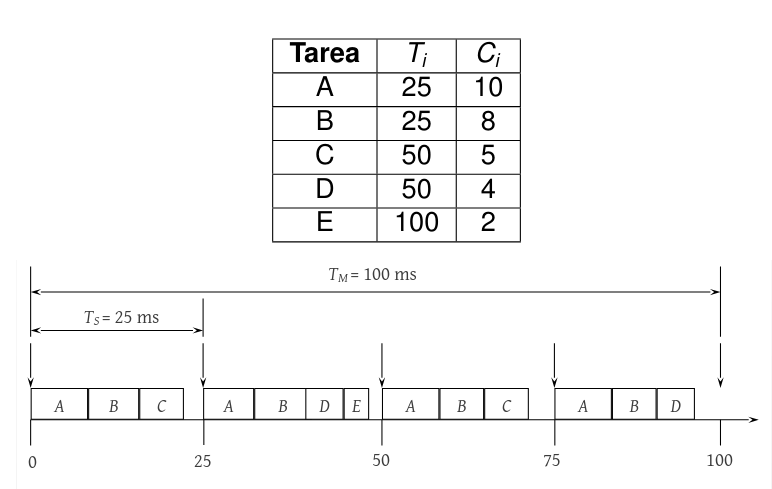
\includegraphics[width=0.6\textwidth]{images/ciclico.png}
    \caption{Planificación cíclica}
    \label{fig:ciclico}
\end{figure}

\subsubsection{Ideas Fundamentales de la Planificación Cíclica}

En la planificación cíclica, el plan principal de ejecución de las tareas es explícito y se define fuera de línea (``off-line''), es decir, sin acceso concurrente al procesador según la prioridad de cada tarea. Las tareas están definidas en un ciclo con una estructura fija.

Algunas características clave de la planificación cíclica son:
\begin{itemize}
    \item El plan principal establece de antemano cómo se entrelazan las tareas en cualquier ejecución del programa, aunque la ordenación relativa de las tareas puede variar en cada ciclo secundario.
    \item Cada tarea se ejecuta completamente una sola vez dentro de cada repetición de su período.
    \item Si una tarea se inicia dentro de una iteración del ciclo secundario, debe terminar antes del final de esa iteración.
\end{itemize}

\subsubsection{Implementación de la Planificación Cíclica}

A continuación se muestra un ejemplo de implementación en C++ para la planificación cíclica:

\begin{lstlisting}[style=customcpp]
void EjecutivoCiclico()
{
    const milliseconds tmp_secundario(25);
    const int nciclos = 4; // Número de ciclos secundarios
    auto siguiente_instante = clock::now();
    int frame = 0; // Número del siguiente ciclo secundario

    while (true) {
        for (frame = 1; frame <= nciclos; frame++) { // Ejecuta las tareas del ciclo secundario actual
            switch (frame) {
                case 0: A(); B(); C(); break;
                case 1: A(); B(); D(); E(); break;
                case 2: A(); B(); C(); break;
                case 3: A(); B(); D(); break;
            }
            siguiente_instante += tmp_secundario; // Pasar al siguiente ciclo secundario
            sleep_until(siguiente_instante); // Esperar inicio siguiente periodo de 25 miliseg.
        }
    }
}
\end{lstlisting}

Cada iteración del bucle \texttt{for} ejecuta un ciclo secundario, y cada 4 iteraciones del bucle se ejecuta un ciclo principal.

\subsubsection{Diseño del Ejecutivo Cíclico}

Para obtener un buen valor de \(T_S\) (duración del ciclo secundario), es necesario considerar algunas restricciones:

\begin{itemize}
    \item El período del ciclo secundario debe ser un divisor del período del ciclo principal, es decir, existe un entero \(k\) tal que: 
    \[
    T_M = k \cdot T_S
    \]
    \item El valor de \(T_S\) debe ser al menos el tiempo de cómputo máximo (\(C_w\)) de cualquier tarea, es decir, \(T_S \geq \max(C_1, C_2, \dots, C_n)\).
    \item \(T_S\) debe ser menor o igual que el mínimo plazo de respuesta máximo (\(D\)) de todas las tareas, es decir, \(T_S \leq \min(D_1, D_2, \dots, D_n)\).
\end{itemize}

Así, el ciclo secundario debe cumplir la siguiente restricción:

\[
\max(C_1, C_2, \dots, C_n) \leq T_S \leq \min(D_1, D_2, \dots, D_n)
\]

\subsubsection{Propiedades del Ejecutivo Cíclico}

Entre las principales propiedades del ejecutivo cíclico destacan:

\begin{itemize}
    \item No existe concurrencia en la ejecución: Cada ciclo secundario es una secuencia de llamadas a procedimientos, sin necesidad de lanzar la ejecución de las tareas.
    \item No es necesario un sistema operativo multitarea ni un núcleo de ejecución en tiempo real.
    \item Los procedimientos acceden secuencialmente a los datos compartidos entre tareas, lo que elimina la necesidad de mecanismos de exclusión mutua (como semáforos o monitores).
    \item No es necesario realizar un análisis de planificabilidad del conjunto de tareas, ya que el sistema es correcto por construcción.
\end{itemize}

\subsubsection{Problemas del Ejecutivo Cíclico}

Sin embargo, la planificación cíclica presenta ciertos problemas, entre los cuales se incluyen:

\begin{itemize}
    \item Dificultad para incorporar tareas con períodos largos.
    \item Las tareas esporádicas son difíciles de tratar, aunque se podría utilizar un servidor de consulta para gestionar su activación.
    \item El plan cíclico es difícil de construir cuando los períodos son de diferentes órdenes de magnitud, lo que hace que el número de ciclos secundarios sea muy grande.
    \item Puede ser necesario dividir una tarea en varios procedimientos.
    \item La planificación es poco flexible y difícil de mantener: cualquier cambio en las tareas implica rehacer toda la planificación.
\end{itemize}

\subsection{Esquema de Planificación de Tareas}

\subsubsection{Determinación de la Planificabilidad de un Conjunto de Tareas}

La planificación de tareas se refiere al proceso de asignar el acceso de las tareas a los procesadores. Para determinar si un conjunto de tareas puede ejecutarse correctamente, se utilizan dos enfoques principales:

\begin{itemize}
    \item \textbf{Algoritmo de planificación}: Determina el orden en que las tareas acceden a los procesadores.
    \item \textbf{Método de análisis de planificabilidad}: Se basa en un test que predice si las tareas son planificables conjuntamente, teniendo en cuenta las condiciones y restricciones especificadas a priori. Este análisis se realiza durante:
    \begin{itemize}
        \item Todas las activaciones posibles de las tareas en su ejecución.
        \item La ejecución de estas tareas, suponiendo la situación más desfavorable, es decir, el \textit{WCET} (Worst Case Execution Time) para cada tarea.
    \end{itemize}
\end{itemize}

\subsubsection{Modelo Simple de Tareas}

El modelo simple de tareas se basa en las siguientes suposiciones:

\begin{itemize}
    \item \textbf{Programa}: Conjunto fijo de tareas que comparten el tiempo de un único procesador.
    \item \textbf{Tareas periódicas}: Con períodos conocidos.
    \item \textbf{Independencia}: Las tareas no se bloquean entre sí al acceder a recursos compartidos.
    \item \textbf{Plazo de respuesta máximo}: Todas las tareas tienen un plazo de respuesta máximo (\(D\)) que coincide con su período (\(T\)).
    \item \textbf{Ignorancia de retrasos del sistema}: Los retrasos debidos al sistema, como los cambios de contexto, son ignorados.
    \item \textbf{Tiempo máximo de cómputo}: El tiempo máximo de ejecución de las tareas (\(C_i\)) es conocido y fijo.
    \item No se contemplan tareas esporádicas ni aperiódicas.
\end{itemize}

\subsubsection{Modelo de Tareas-II: Notación}

La notación utilizada para describir las tareas es la siguiente:

\begin{itemize}
    \item \(P\): Prioridad de la tarea (si fuera aplicable).
    \item \(\tau\): Tarea (nombre de la tarea).
    \item \(t_a\): Tiempo de activación (instante en que la tarea está lista para su ejecución).
    \item \(t_s\): Tiempo de comienzo (instante en que la tarea comienza realmente su ejecución).
    \item \(t_f\): Tiempo de finalización (instante en que la tarea finaliza su ejecución).
    \item \(t_l, d\): Tiempo límite (instante límite para la ejecución de la tarea, \(t_l(k) = d = t_a + D\)).
    \item \(T\): Periodo de ejecución (intervalo entre dos activaciones sucesivas de una tarea periódica).
    \item \(J\): Latencia (tiempo entre la activación y el inicio de la ejecución de la tarea, \(J(k) = t_s(k) - t_a(k)\)).
    \item \(C\): Tiempo de cómputo (tiempo de ejecución de la tarea).
    \item \(C_{\text{max}}\): Cómputo máximo (tiempo de ejecución en el peor caso de la tarea).
    \item \(e\): Tiempo transcurrido (tiempo entre el comienzo y la finalización de la tarea, \(e(k) = t_f(k) - t_s(k)\)).
    \item \(R\): Tiempo de respuesta (tiempo total para completar la ejecución de la tarea, \(R(k) = J(k) + e(k)\)).
\end{itemize}

\subsubsection{Propósito de la Planificación de Tareas}

La planificación de tareas, o \textit{task-scheduling}, estudia técnicas de Programación Entera para obtener una asignación eficiente de recursos y tiempo a las actividades. El objetivo es cumplir ciertos requisitos de eficiencia, utilizando heurísticas que maximicen la función objetivo \(U(N)\), que representa la utilización del procesador para \(N\) tareas de tiempo real.

\subsubsection{Planificación con Prioridades}

La planificación con prioridades permite solucionar los problemas mencionados previamente. Cada tarea tiene asociada un valor entero positivo, conocido como la prioridad de la tarea, que refleja su importancia relativa en el conjunto de tareas. Las principales características de la planificación con prioridades incluyen:

\begin{itemize}
    \item La prioridad se asigna en función de las necesidades temporales de la tarea, no de su rendimiento o comportamiento.
    \item Las tareas ejecutables se despachan para su ejecución en orden de prioridad.
    \item La prioridad de una tarea puede depender de su \textit{urgencia}, pero no de su \textit{criticidad} en términos de tiempo real.
\end{itemize}

\subsubsection{Esquema de Planificación de Tareas}

El esquema de planificación de tareas generalmente consta de los siguientes elementos:

\begin{enumerate}
    \item Un algoritmo para ordenar el acceso de las tareas al procesador.
    \item Un test para predecir el comportamiento del sistema en el peor caso de planificación, es decir, cuando existe mayor interferencia entre las tareas.
    \item Características principales de un esquema de planificación de tareas de tiempo real:
    \begin{itemize}
        \item Dinámico vs. estático.
        \item Desplazante (preemptive) de tareas menos prioritarias.
        \item Análisis de tareas dentro de una "ventana temporal".
        \item Concepto de instante crítico.
    \end{itemize}
    \item Una posible solución al problema de análisis temporal de las tareas esporádicas y aperiódicas.
\end{enumerate}

\subsubsection{Planificación con Prioridades-II: Tipos de Esquemas}

Existen dos tipos de esquemas de planificación con prioridades:

\begin{itemize}
    \item \textbf{Prioridades asignadas estáticamente a las tareas}: Cada tarea tiene una prioridad fija durante toda la ejecución del sistema.
    \begin{itemize}
        \item \textit{Cadencia monótona o RMS (Rate Monotonic Scheduling)}: La prioridad se asigna a la tarea con el período más corto (mayor frecuencia de activación).
        \item \textit{Plazo de respuesta monótono o DMS (Deadline Monotonic Scheduling)}: Se asigna mayor prioridad a la tarea con el plazo de respuesta más corto.
    \end{itemize}
    \item \textbf{Prioridades asignadas dinámicamente a las tareas}: Las prioridades de las tareas cambian durante la ejecución del sistema.
    \begin{itemize}
        \item \textit{EDF (Earliest Deadline First)}: Se asigna prioridad a la tarea cuyo plazo de respuesta absoluto es más cercano.
        \item \textit{LLF (Least Laxity First)}: Se asigna prioridad a la tarea con menor holgura temporal.
    \end{itemize}
\end{itemize}

\subsubsection{Modelo de Tareas-IV: Notación Adicional}

Se introducen más parámetros de interés en la planificación de tareas:

\begin{itemize}
    \item \(D\): Plazo de respuesta máximo.
    \item \(\varphi\): Desplazamiento o fase, el tiempo para activarse por primera vez.
    \item \(RJ\): Fluctuación relativa o jitter, la máxima desviación en el tiempo de comienzo entre dos activaciones sucesivas de una tarea, definida como:
    \[
    RJ = \max((t_s(k+1) - t_a(k+1)) - (t_s(k) - t_a(k)))
    \]
    \item \(H\): Holgura o slack time, el tiempo disponible para permanecer activa dentro del plazo de respuesta máximo:
    \[
    H(k) = t_l - t_a(k) - e(k) = D - e(k)
    \]
\end{itemize}


\subsection{Esquema de Planificación de Tareas de Tiempo Real Basado en el Algoritmo de Cadencia Monótona (RMS)}

\subsubsection{1. Algoritmo de Cadencia Monótona (Rate Monotonic Scheduling)}

El algoritmo de cadencia monótona (RMS)\footnote{Para un ejemplo de ello accede  a la diapositiva 4.39 del tema 4} se basa en los siguientes principios:

\begin{itemize}
    \item Las prioridades se asignan de manera estática a cada tarea (\(\tau_i\)).
    \item La prioridad es mayor para las tareas con menor período (\(T_i\)):
    \[
    \forall i, j : T_i < T_j \implies P_i > P_j
    \]
    \item Este algoritmo no tiene en cuenta la criticidad de las tareas, sino su urgencia, definida como \( \frac{1}{T_i} \).
    \item El RMS es óptimo entre los algoritmos de asignación estática de prioridades bajo las siguientes condiciones:
    \begin{itemize}
        \item Las tareas son periódicas.
        \item El plazo de respuesta de cada tarea coincide con su período (\(D_i = T_i\)).
    \end{itemize}
\end{itemize}

\subsubsection{2. Test de Planificabilidad Basado en el Factor de Utilización del Procesador}

El test de planificabilidad para un conjunto de tareas periódicas \(\{\tau_1, \tau_2, \ldots, \tau_N\}\) verifica la suma del factor de utilización del procesador:

\[
U = \sum_{i=1}^N \frac{C_i}{T_i}
\]

\begin{itemize}
    \item En un sistema de \(N\) tareas periódicas, independientes y con prioridades asignadas según su frecuencia (inverso al período), el sistema es planificable si el factor de utilización del procesador (\(U(N)\)) cumple la siguiente condición:
    \[
    U = \sum_{i=1}^N \frac{C_i}{T_i} < U_0 = N \cdot (2^{\frac{1}{N}} - 1)
    \]
    \item Si \(U \leq U_0(N)\), el sistema es planificable. En caso contrario, el test no puede determinar si el sistema es planificable (es una condición suficiente, pero no necesaria).
\end{itemize}

\subsubsection{3. Inexactitud del Test de Planificabilidad RM}

El límite máximo de utilización \(U_0(N)\) depende del número de tareas \(N\) y decrece conforme aumenta \(N\). A continuación, se muestran algunos valores:

\begin{table}[H]
\centering
\begin{tabular}{|c|c|}
\hline
\textbf{\(N\)} & \textbf{\(U_0(N)\) (\%)} \\
\hline
1 & 100 \\
2 & 82.85 \\
3 & 78.0 \\
4 & 75.7 \\
5 & 74.3 \\
10 & 71.8 \\
\(\infty\) & 69.3 \\
\hline
\end{tabular}
\caption{Límite máximo de utilización del procesador \(U_0(N)\) en función del número de tareas \(N\).}
\end{table}

\subsubsection{4. Características del Test RMS}

\begin{itemize}
    \item El test basado en el factor de utilización es solo una condición suficiente para determinar si un conjunto de tareas es planificable.
    \item En caso de que un conjunto de tareas no pase el test, es posible realizar un análisis más detallado utilizando diagramas de Gantt en una ventana temporal definida como:
    \[
    M_i = \text{m.c.m.}\{T_1, T_2, \ldots, T_i\}
    \]
    \item Los tests de planificabilidad basados en la utilización del procesador no proporcionan información sobre los tiempos de respuesta de las tareas.
\end{itemize}

\subsection{Segundo Teorema de Planificabilidad de un Conjunto de Tareas Periódicas}

El segundo teorema de planificabilidad establece las siguientes condiciones para un sistema de \(N\) tareas periódicas independientes, con prioridades asignadas en orden de su frecuencia (menor período, mayor prioridad):

\begin{itemize}
    \item Todas las tareas cumplen sus tiempos límite si, cuando se activan simultáneamente, cada tarea finaliza su ejecución antes de que expire el tiempo límite asignado en su primera activación.
    \item Con este criterio, se puede alcanzar una utilización máxima del procesador:
    \[
    \sum_{i=1}^N \frac{C_i}{T_i} \leq 1
    \]
\end{itemize}

\subsubsection{Características del Segundo Teorema}

\begin{itemize}
    \item La cota máxima que puede alcanzar el factor de utilización (\(U\)) es ahora mayor que la permitida por el test RMS.
    \item Este test es más flexible y puede aplicarse a un mayor número de conjuntos de tareas, ya que permite un mayor factor de utilización del procesador.
    \item A diferencia del test de RMS, este test es exacto:
    \begin{itemize}
        \item Proporciona una condición necesaria y suficiente para determinar si un conjunto de tareas es planificable.
        \item Si las tareas pasan este test, el sistema es planificable en todos los casos.
    \end{itemize}
\end{itemize}

\subsection{Ventajas de los Esquemas de Planificación Estáticos}

Los esquemas de planificación estáticos presentan varias ventajas importantes:

\begin{itemize}
    \item \textbf{Simplicidad y eficiencia}: 
    \begin{itemize}
        \item Son más sencillos y eficientes de implementar en comparación con los esquemas dinámicos.
        \item Requieren menos recursos computacionales para su ejecución.
    \end{itemize}
    \item \textbf{Facilidad de diseño}: 
    \begin{itemize}
        \item Es más sencillo diseñar un sistema con tiempos límite (plazos de respuesta absolutos) calculados exactamente.
    \end{itemize}
    \item \textbf{Flexibilidad}: 
    \begin{itemize}
        \item Permiten la incorporación de otros factores que influyen en la planificación de tareas, especialmente cuando las prioridades no están directamente asociadas a los tiempos límite.
    \end{itemize}
    \item \textbf{Predictibilidad bajo sobrecarga transitoria}:
    \begin{itemize}
        \item Durante períodos de sobrecarga transitoria, los esquemas estáticos suelen ser más predecibles.
        \item Esto no siempre es cierto en los esquemas dinámicos, como el algoritmo \textit{Earliest Deadline First} (EDF\footnote{Ejemplo en la diapositiva 4.44 del tema 4}).
    \end{itemize}
\end{itemize}

\subsection{Modelo General de Tareas de Tiempo Real (TR)}

La estructura general asumida para resolver el problema de planificabilidad incluye las siguientes características:

\begin{itemize}
    \item \textbf{Programa:} Conjunto fijo de tareas que comparten el tiempo de un procesador. Pueden incluirse tareas aperiódicas o esporádicas.
    \item \textbf{Bloqueo:} Las tareas pueden bloquearse al acceder a recursos compartidos, como semáforos utilizados en su código.
    \item \textbf{Plazo de respuesta máximo (\(D\)):} 
    \begin{itemize}
        \item Generalmente, no coincide con su período (\(T\)).
        \item En el caso de las tareas esporádicas, el plazo de respuesta máximo suele ser muy corto.
    \end{itemize}
    \item \textbf{Simplificaciones:}
    \begin{itemize}
        \item Se ignoran los retrasos debidos al sistema (como cambios de contexto).
        \item No se guardan eventos de tiempo real.
        \item El tiempo máximo de cómputo de las tareas (\(C\)) se considera conocido y fijo.
    \end{itemize}
\end{itemize}

\subsection{Inversión de Prioridad}

\subsubsection{Descripción del Problema}

El problema de la inversión de prioridad ocurre en los siguientes casos:

\begin{itemize}
    \item Una tarea más prioritaria queda bloqueada y debe esperar arbitrariamente largo tiempo debido a la ejecución continua de tareas menos prioritarias.
    \item Esto invalida cualquier previsión sobre la planificación del conjunto de tareas, incluso si han pasado el test de planificabilidad como el RMS.
    \item Surge como consecuencia del esquema estático de asignación de prioridades a las tareas.
\end{itemize}

\subsubsection{Características de la Inversión de Prioridad}

\begin{itemize}
    \item La inversión de prioridad no puede eliminarse completamente, pero sus efectos adversos sobre la planificación pueden minimizarse.
\end{itemize}

\subsection{Protocolo de Sección Crítica No Expulsable}

\subsubsection{Descripción del Protocolo}

\begin{itemize}
    \item Durante la ejecución de las secciones críticas, las tareas tienen una prioridad estática igual a la prioridad máxima del sistema.
\end{itemize}

\subsubsection{Características del Protocolo}

\begin{itemize}
    \item Es el protocolo más simple para evitar la inversión de prioridad.
    \item Puede inducir bloqueos excesivamente largos en las tareas más prioritarias.
    \item En ciertos casos, puede interferir con la ejecución de todas las tareas, incluso si estas no hacen uso de recursos compartidos.
\end{itemize}

\subsection{Tiempo de Bloqueo en Sección Crítica No Expulsable}

\begin{itemize}
    \item Para una tarea \(\tau_i\), el tiempo de ejecución en el peor caso se incrementará por un factor constante:
    \[
    C_i^* = C_i + B_i
    \]
    \item La tarea más prioritaria \(\tau_i\) puede ser bloqueada, como máximo, durante la ejecución de una única sección crítica:
    \[
    B_i = \max_{j, j > i} \left( \max_k \text{Dur}(s_{jk}) \right)
    \]
    \item Aquí:
    \begin{itemize}
        \item \(s_{jk}\) representa la sección crítica \(k\) ejecutada por la tarea \(\tau_j\), que tiene menor prioridad que \(\tau_i\).
        \item \(\text{Dur}(s_{jk})\) es la duración de dicha sección crítica.
    \end{itemize}
\end{itemize}

\subsection{Protocolo de Herencia de Prioridad}

\subsubsection{Descripción del Protocolo}

El protocolo de herencia de prioridad se basa en el siguiente principio\footnote{Ejemplo de esto se encuentra en la diapositiva 4.52 del tema 4}:

\begin{itemize}
    \item La \textbf{prioridad efectiva} de una tarea en ejecución será el máximo entre:
    \begin{itemize}
        \item Su \textbf{prioridad por defecto}, asignada al inicio del programa.
        \item Las \textbf{prioridades} de otras tareas con las que comparte recursos y que mantiene bloqueadas en ese momento.
    \end{itemize}
\end{itemize}

\subsubsection{Características del Protocolo}

\begin{itemize}
    \item Las prioridades de las tareas no son estáticas; pueden variar dinámicamente durante la ejecución del programa.
    \item Este enfoque permite:
    \begin{itemize}
        \item \textbf{Minimizar el efecto de la inversión de prioridad}: 
        Al elevar temporalmente la prioridad de las tareas bloqueadas, se evita que estas queden en espera indefinidamente.
        \item \textbf{Optimizar el aprovechamiento del procesador}: 
        Se prioriza la resolución de bloqueos en recursos compartidos, reduciendo el tiempo total de ejecución.
    \end{itemize}
\end{itemize}

\subsubsection{Ventajas del Protocolo}

\begin{itemize}
    \item Reducción de los bloqueos prolongados.
    \item Mayor predictibilidad en la planificación de tareas.
    \item Mejor utilización de los recursos del sistema.
\end{itemize}







\subsection{Tipos de Bloqueos en el Protocolo de Herencia de Prioridad}

\subsubsection{Tipos de Bloqueos}
Con el protocolo de herencia de prioridad, se identifican los siguientes tipos de bloqueos:
\begin{enumerate}[label=\alph*)]
    \item \textbf{Bloqueos directos:} Ocurren cuando una tarea de mayor prioridad se encuentra bloqueada esperando un recurso compartido que está siendo utilizado por una tarea de menor prioridad.
    \item \textbf{Bloqueos indirectos:} Ocurren cuando una tarea de mayor prioridad es bloqueada debido a que otra tarea de menor prioridad está esperando un recurso bloqueado por una tercera tarea.
\end{enumerate}

\subsubsection{Características del Protocolo}
\begin{itemize}
    \item Las tareas sólo pueden ser bloqueadas un número limitado de veces por otras tareas de menor prioridad.
    \item Consecuencias:
    \begin{enumerate}
        \item Si una tarea tiene definidas \(M\) secciones críticas, entonces el número máximo de veces que puede ser bloqueada es \(M\).
        \item Si hay \(N < M\) tareas de menor prioridad, el número máximo de bloqueos se reduce a \(N\).
    \end{enumerate}
\end{itemize}

\subsection{Cálculo del Factor de Bloqueo}

El factor de bloqueo (\(B_i\)) para una tarea \(\tau_i\) está dado por el mínimo entre dos términos:

\begin{enumerate}
    \item \(Bl_i:\) Bloqueo debido a tareas \(\tau_j\) menos prioritarias que acceden a secciones críticas \(k\) compartidas con tareas de mayor prioridad:
    \[
    Bl_i = \sum_{j=i+1}^{n} \max_k[Dur_{j,k} : Limite(S_k) \geq P_i]
    \]

    \item \(Bs_i:\) Bloqueo debido a todas las secciones críticas a las que accede la tarea \(\tau_i\):
    \[
    Bs_i = \sum_{k=1}^{m} \max_{j>i}[Dur_{j,k} : Limite(S_k) \geq P_i]
    \]
\end{enumerate}

El factor de bloqueo total para la tarea \(\tau_i\) es:
\[
B_i = \min(Bl_i, Bs_i)
\]

\subsection{Protocolos de Techo de Prioridad}

\subsubsection{Techo de Prioridad de un Recurso}
El \textbf{techo de prioridad} de un recurso es la prioridad de la tarea más prioritaria que puede bloquear el acceso al recurso.

\subsubsection{Características de los Protocolos de Techo de Prioridad}
\begin{itemize}
    \item Garantizan que una tarea prioritaria sólo puede ser bloqueada como máximo una vez por otras de menor prioridad.
    \item Previenen los interbloqueos.
    \item Eliminan los bloqueos transitivos.
    \item Aseguran el acceso en exclusión mutua a los recursos compartidos.
\end{itemize}

\subsection{Protocolo de Techo de Prioridad Inmediato (PPP)}

\begin{enumerate}
    \item Cada tarea tiene una \textbf{prioridad estática} asignada por defecto.
    \item Cada recurso tiene un valor de \textbf{techo de prioridad} definido.
    \item Una tarea tiene una \textbf{prioridad dinámica}, que es el máximo entre:
    \begin{itemize}
        \item Su prioridad estática inicial.
        \item Los valores de los techos de prioridad de los recursos que mantiene bloqueados\footnote{Ejemplo del PPP en la diapositiva 4.57 del tema 4}.
    \end{itemize}
\end{enumerate}

\subsection{Tiempo de Bloqueo}

\subsubsection{Cálculo del Tiempo de Bloqueo}
El tiempo máximo de bloqueo de una tarea \(\tau_i\) está dado por la duración de la sección crítica más larga a la que acceden las tareas de prioridad inferior, siempre que el techo de prioridad del recurso sea igual o superior a la prioridad de \(\tau_i\):
\[
B_i = \max_{\{j,k\}} \{Dur_{j,k} \, | \, \text{prio}(\tau_j) < \text{prio}(\tau_i), \, \text{techo\_prioridad}(S_k) \geq \text{prio}(\tau_i)\}
\]

\subsubsection{Comportamiento con el Protocolo de Techo de Prioridad Inmediato (PPP)}
Con el protocolo PPP:
\begin{itemize}
    \item Una tarea puede ser bloqueada por otra de menor prioridad aunque no accedan a recursos comunes.
    \item Esto ocurre debido a la dinámica del techo de prioridad que se asigna a los recursos bloqueados.
\end{itemize}

\subsection{Asignación de Prioridades a las Tareas Aperiódicas}

\begin{itemize}
    \item En aplicaciones de tiempo real, las tareas aperiódicas no deben tener una prioridad inferior a la de las tareas de misión crítica.
    \item Para gestionar las tareas aperiódicas, se utiliza un \textbf{servidor aperiódico}, que puede ser:
    \begin{itemize}
        \item Una tarea real o conceptual.
        \item Diseñado para ejecutar procesos aperiódicos tan pronto como sea posible, sin afectar las garantías de las tareas periódicas.
    \end{itemize}
\end{itemize}

\subsection{Servicio de Tareas Aperiódicas}

\subsubsection{Servicio con Tiempo en Segundo Plano}
\begin{itemize}
    \item El tiempo aperiódico se incrementa a intervalos regulares.
    \item Estas tareas tienen la prioridad más baja del sistema.
    \item Si no hay peticiones aperiódicas, el tiempo asignado a estas tareas se pierde\footnote{Ejemplo en la diapositiva 4.60 del tema 4}.
\end{itemize}

\subsubsection{Servicio de Aperiódicas con Sondeos}
\begin{itemize}
    \item Se incluye una tarea adicional, denominada \textbf{tarea sondeante}, dentro del conjunto de tareas periódicas.
    \item Características de la tarea sondeante:
    \begin{itemize}
        \item Tiene un periodo \(T_s\) y un tiempo de ejecución en el peor caso \(C_s\).
        \item Se le asigna una prioridad adecuada dentro del sistema.
    \end{itemize}
    \item El test de planificabilidad de cadencia monótona se aplica considerando la tarea sondeante\footnote{Ejemplo en la diapositiva 4.62 del tema 4}:
    \[
    \sum_{i=1}^{N} \frac{C_i}{T_i} + \frac{C_s}{T_s} \leq (N + 1)\left(2^{\frac{1}{N+1}} - 1\right)
    \]
\end{itemize}

\subsection{Servidor Diferido}

\subsubsection{Características del Servidor Diferido}
\begin{itemize}
    \item Preserva el tiempo dedicado a tareas aperiódicas, incluso si temporalmente no hay peticiones de este tipo.
    \item Se asigna un tamaño de servidor \(C_s\) que se utiliza únicamente para atender peticiones aperiódicas.
    \item El tamaño del servidor \(C_s\) se recarga hasta su valor máximo al inicio de cada periodo del servidor \(T_s\).
    \item El valor inicial de \(C_s\) se establece tras un análisis previo de planificabilidad del conjunto de tareas.
    \item Las peticiones aperiódicas se atienden con una prioridad alta, siempre que el tiempo del servidor no se haya agotado.
\end{itemize}

\subsubsection{Análisis de Planificabilidad con el Servidor Diferido}

\subsubsubsection{Configuración del Sistema}
\begin{itemize}
    \item Conjunto de \(N\) tareas periódicas: \(\tau_1, \tau_2, \dots, \tau_N\).
    \item Un servidor diferido con prioridad más alta, y un tamaño \(C_s\) asociado a un periodo \(T_s\).
\end{itemize}

\subsubsubsection{Cálculo del Límite Superior de Utilización}
El límite superior de utilización se calcula como:
\[
U_{\text{mls}} = U_s + N \left[\left(\frac{U_s + 2}{2U_s + 1}\right)^{\frac{1}{N}} - 1\right]
\]

\textbf{Límite cuando \(N \to \infty\):}
\[
\lim_{N \to \infty} U_{\text{mls}} = U_s + \ln\left(\frac{U_s + 2}{2U_s + 1}\right)
\]

\subsubsubsection{Condición de Planificabilidad}
Para un conjunto de \(N\) tareas periódicas y un servidor diferido con límites de utilización \(U_p\) y \(U_s\), respectivamente, se garantiza la planificabilidad con el algoritmo de cadencia monótona si:
\[
U_p + U_s \leq U_{\text{mls}}
\]

\textbf{Forma equivalente:}
\[
U_p \leq \ln\left(\frac{U_s + 2}{2U_s + 1}\right)
\]

\subsubsection{Ventajas del Servidor Diferido}
\begin{itemize}
    \item Maximiza el tiempo disponible para las tareas aperiódicas.
    \item Permite una respuesta eficiente a las tareas aperiódicas con prioridad alta.
    \item Reduce el impacto de las tareas aperiódicas en la planificación de las tareas periódicas\footnote{Ejemplo del servidor diferido en la diapositiva 4.65 del tema 4}.
\end{itemize}




\end{document}
